%----------------------------------------------------------------------------------------
%	PACKAGES AND THEMES
%----------------------------------------------------------------------------------------
\PassOptionsToPackage{table}{xcolor}
\documentclass[aspectratio=169,xcolor=dvipsnames,svgnames,x11names,fleqn]{beamer}
% \documentclass[aspectratio=169,xcolor=dvipsnames,fleqn]{beamer}

\usetheme{RedVelvet}

\usefonttheme[onlymath]{serif}
\usepackage{xspace}
\usepackage{amsmath}
\usepackage{amssymb}
\usepackage{amsfonts}
\usepackage{color}
\usepackage{physics}
% \usepackage{mathbb}
\usepackage{rahul_math}
\usepackage{bigints}
\usepackage{hyperref}
\hypersetup{
  colorlinks,
  citecolor=Violet,
  linkcolor=Black}
\usepackage{graphicx} % Allows including images
\usepackage{booktabs} % Allows the use of \toprule, \midrule and \bottomrule in tables
\usepackage{tikz,pgfplots}
\usepackage{subfigure}
\usetikzlibrary{arrows}
\usepackage{minted}
\definecolor{LightGray}{gray}{0.9}
\definecolor{cream}{rgb}{0.92, 0.9, 0.55}
\definecolor{lightblue}{rgb}{0.68, 0.85, 0.9}


\usepackage{xcolor-material}
\usetikzlibrary{fit}
\tikzset{%
apple/.pic={
  \fill [MaterialBrown] (-1/8,0)  arc (180:120:1 and 3/2) coordinate [pos=3/5] (@)-- ++(1/6,-1/7)  arc (120:180:5/4 and 3/2) -- cycle;
  \fill [MaterialLightGreen500] (0,-9/10)  .. controls ++(180:1/8) and ++(  0:1/4) .. (-1/3,  -1) .. controls ++(180:1/3) and ++(270:1/2) .. (  -1,   0) .. controls ++( 90:1/3) and ++(180:1/3) .. (-1/2, 3/4) .. controls ++(  0:1/8) and ++(135:1/8) .. (   0, 4/7)
}
}

\usepackage{tikz}

\newcommand{\redcircle}[1]{%
    \tikz[baseline=(char.base)]{
        \node[shape=circle,inner sep=1.75pt,fill=roseRed,text=white] (char) {#1};
    }
}


\newcommand{\leftdoublequote}{\textcolor{blue}{\scalebox{3}{``}}}

\newcommand{\rightdoublequote}{\textcolor{blue}{\scalebox{3}{''}}}


\usepackage{textcomp}
\usepackage{fontawesome}

\usepackage{overpic}

%----------------------------------------------------------------------------------------
%	TITLE PAGE
%----------------------------------------------------------------------------------------

\usepackage{tikz-qtree,tikz-qtree-compat}
\usetikzlibrary{calc}


\title[CPE 381: Signals and Systems]{CPE 381: Fundamentals of Signals and Systems for Computer Engineers} % The short title appears at the bottom of every slide, the full title is only on the title page
\subtitle{02 Continuous \& Discrete Representation}

\author[Rahul Bhadani] {{\Large \textbf{Rahul Bhadani}}}

\institute[UAH] % Your institution as it will appear on the bottom of every slide, maybe shorthand to save space
{
    Electrical \& Computer Engineering,  The University of Alabama in Huntsville
}
\date

% \titlegraphic{
%    \includegraphics[width=0.4\linewidth]{figures/UAH_primary.png}
% }

\begin{document}

%-------------------------------------------------
\begin{frame}
  \titlepage
\end{frame}

%-------------------------------------------------
\begin{frame}{Outline}
   \tableofcontents
\end{frame}



\section{Continuous and Discrete Representations}

\begin{frame}{}
    \begin{center}
    \Huge \bf \color{DarkBlue}
    \faFire
    
Continuous and Discrete Representations
\end{center}
\end{frame}

\begin{frame}{Continuous and Discrete Representations}
    \begin{itemize}
        \item \textbf{Continuous-time signals:} Depend continuously on time.
        \item \textbf{Discrete-time signals:} Sequences of measurements typically made at uniform times.
        \item \textbf{Sampling process:} 
        \begin{equation*}
            x[n] = x(nT_s) = x(t)|_{t=nT_s}
        \end{equation*}
        \item \textbf{Example:} 
        \begin{itemize}
            \item Analog signal: $$ x(t) = 2 \cos(2\pi t) $$
            \item Sampled at $ T_{s1} = 0.1 $ s: $ x_1[n] = 2 \cos(2\pi n/10) $
            \item Sampled at $ T_{s2} = 1 $ s: $ x_2[n] = 2 \cos(2\pi n) = 2 $
        \end{itemize}
        \item \textbf{Key point:} Choosing an appropriate sampling period \( T_s \) is crucial to preserve information.
    \end{itemize}
\end{frame}
\begin{frame}{Sampling Continuous Time Signals}
    \centering
    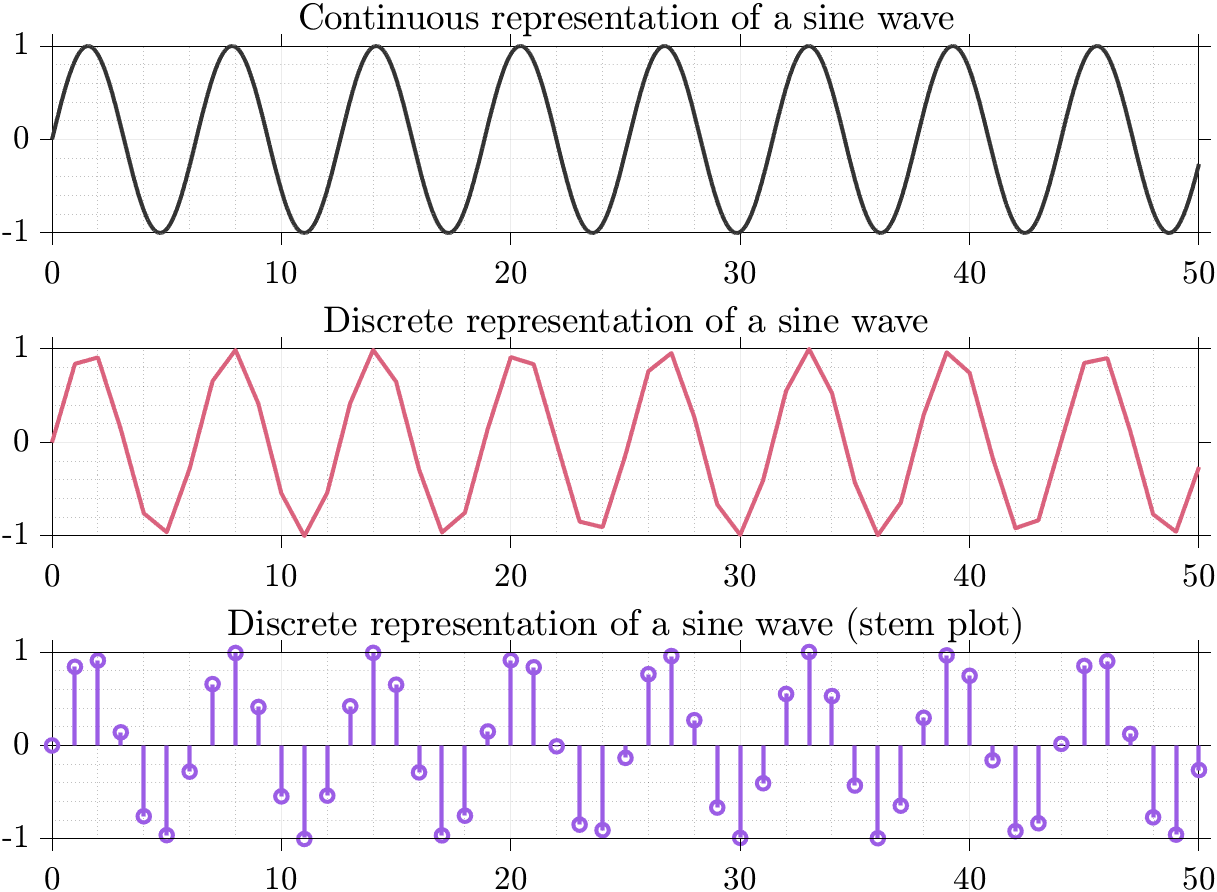
\includegraphics[width=0.45\linewidth, trim=0 0 0 0cm,clip]{figures/sampled_sine_wave.png} 
    
    $x[n] = x(nT_s)$,
$T_s$ = sample time.
    
    \tiny
    Code for the figure: \url{https://github.com/rahulbhadani/CPE381_FA25/blob/main/Code/sampled_sine_wave.m}
\end{frame}

\begin{frame}{Sampling Process}
    \begin{itemize}
        \item \( x[n] = x(nT_s) = x(t)|_{t=nT_s} \)
        \item This equation represents the \textbf{sampling process} where a continuous-time signal \( x(t) \) is sampled at uniform intervals \( T_s \) to produce a discrete-time signal \( x[n] \).
        \item \textbf{Key Points:}
            \begin{itemize}
                \item \( n \) is an integer representing the sample index.
                \item \( T_s \) is the sampling period.
                \item The continuous-time signal \( x(t) \) is sampled at \( t = nT_s \).
            \end{itemize}
    \end{itemize}
\end{frame}

\begin{frame}
\frametitle{Derivatives and Finite Differences}
\textbf{Continuous-Time Derivatives:}
\begin{itemize}
    \item Derivatives measure the rate of change of a function.
    \item Defined as the limit of the difference quotient as the interval approaches zero.
    \item Represented as \( \frac{dy}{dt} \) for a function \( y(t) \).
\end{itemize}
\end{frame}

\begin{frame}
\frametitle{Finite Differences}
\textbf{Discrete-Time Derivatives:}
\begin{itemize}
    \item Finite differences approximate derivatives for discrete-time signals.
    \item Forward difference: \( \Delta x[n] = x[n+1] - x[n] \).
    \item Backward difference: \( \Delta x[n] = x[n] - x[n-1] \).
\end{itemize}
\vspace{5pt}
$x[n] = x(nT_s)$ when looking at continuous to discrete domain where $T_s$ is the sampling time, $n$ is any positive integer. We will look at this much later in detail.
\end{frame}

\begin{frame}
\frametitle{Central Differences}
\textbf{Central Difference:}
\begin{itemize}
    \item Provides a more accurate approximation.
    \item Defined as \( \delta x[n] = \frac{x[n+1] - x[n-1]}{2} \).
    \item Reduces error compared to forward and backward differences.
\end{itemize}
\end{frame}


\begin{frame}{Relation between the Derivative and Finite Difference}
    The derivative and the finite-difference operators are not the same. In the limit, we have:
    \begin{equation*}
            \frac{dx(t)}{dt}|_{t = nT_s} = \lim_{T_s\to 0 }\cfrac{\Delta [x (nT_s)]}{T_s}
    \end{equation*}

\end{frame}

\begin{frame}
\frametitle{Applications}
\textbf{Applications of Finite Differences:}
\begin{itemize}
    \item Used in numerical methods for solving differential equations.
    \item Essential in digital signal processing and control systems.
    \item Helps in approximating continuous-time derivatives in discrete systems.
\end{itemize}
\end{frame}

\begin{frame}{Discrete Integration}
Recall, the integration in the continuous domain is 
$$
I(t) = \int_{t_0}^t x(\tau) d\tau
$$
then, we have 
$$
\cfrac{d}{dt} \int_{t_0}^t x(\tau) d\tau = x(t)
$$

If we use $D$ for the derivative operator, then $D^{-1}$ is the integration operator.

$$
D[ D^{-1}[x(t)]] = x(t))
$$
\end{frame}

\begin{frame}
\frametitle{Example}
\begin{columns}
\column{0.5\linewidth}
    \begin{itemize}
    \item Computational integration using sums:
    $$
    \int_{0}^{10} t \, dt = \frac{t^2}{2} \bigg|_{0}^{10} = 50
    $$
\end{itemize}
\column{0.5\linewidth}
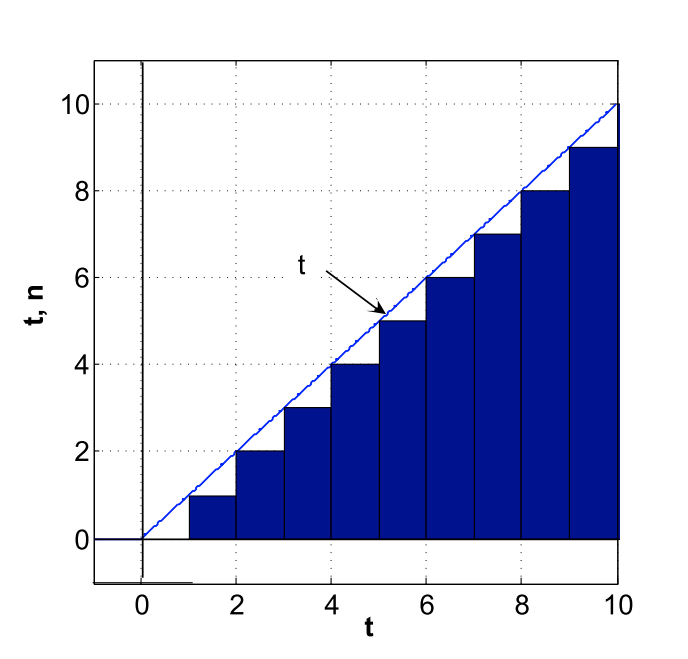
\includegraphics[width=0.7\linewidth, trim=0 0 0 0cm,clip]{figures/slopeline.png} 
\end{columns}

\end{frame}

\begin{frame}
\frametitle{Discrete Approximation}
\begin{columns}
\column{0.5\linewidth}
\begin{itemize}
    \item Approximation using pulses ($T_s = 1$)(rectangle of width $T_s = 1$, height = $n$):
    $$
    \sum_{n=0}^{9} p[n] = \sum_{n=0}^{9} n = 45
    $$
    \item Generalized sum:
    $$
    \sum_{n=0}^{N-1} n = \frac{N \times (N-1)}{2}
    $$
\end{itemize}
\column{0.5\linewidth}
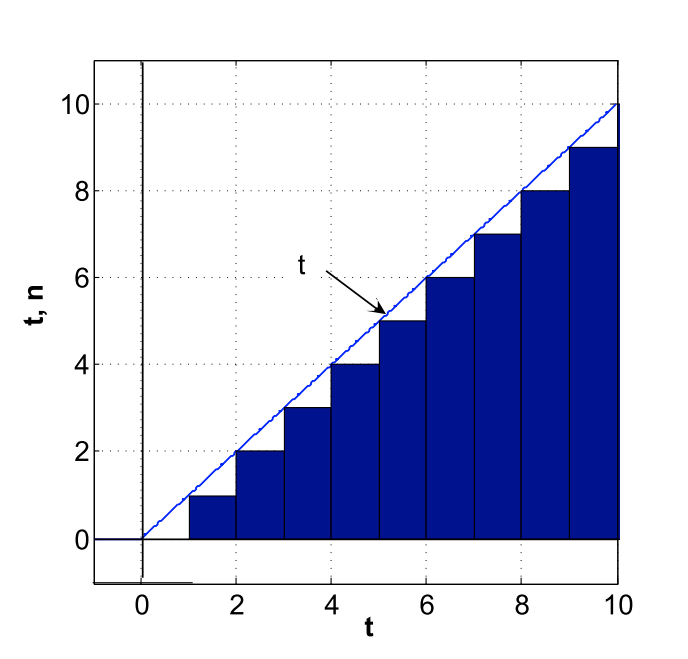
\includegraphics[width=0.7\linewidth, trim=0 0 0 0cm,clip]{figures/slopeline.png} 
\end{columns}


\end{frame}

\begin{frame}
\frametitle{Improved Discrete Approximation}
\begin{itemize}
    \item Using \( T_s = 10^{-3} \):
    $$
    \sum_{n=0}^{(10/T_s)-1} nT_s^2 = \sum_{n=0}^{(10/T_s)-1} n 10^{-6} = 49.995
    $$
    The height of each pulse is $nT_s$ and the width is $T_s$.
\end{itemize}

Hence, the sampling time (or its inverse -- sampling frequency matters).
\end{frame}


\section{Numerical Computation in MATLAB}



\begin{frame}{}
    \begin{center}
    \Huge \bf \color{DarkBlue}
    \faFire
    
Numerical Computation in MATLAB

\end{center}
\end{frame}


\begin{frame}[containsverbatim]{Signal Generation in MATLAB}

\begin{enumerate}
\item Choosing time-points
\item Uniformly sampled (ideal) vs non-uniformly sampled (real-life)
\item Specification: frequency, or sampling-time
\item Specify function
\item We primarily study uniformly-sampled signals in this course.
\end{enumerate}

\end{frame}

\begin{frame}[containsverbatim]{Example in MATLAB}

   \begin{tblock}{}

        \begin{minted}
            [
            framesep=1mm,
            baselinestretch=1.2,
            fontsize=\footnotesize
            ]
            {matlab}
%% Signal with Fixed Sampling-time
sampling_time = 0.5; % 0.5 seconds
final_time = 10; % 10 seconds
% Generate time points on which to evaluate the function
t = 0:sampling_time:final_time;
x = sin(t);
% Plotting
f = figure;
f.Position = [744   358   914   592]; % Position of figure on the screen
hold on;
plot(t, x, 'LineStyle','-', 'LineWidth',2,'Marker','o', ...
    'Color','#426642', ...
    'DisplayName', 'Sine Wave with Uniform Sampling');
        \end{minted}

    \end{tblock}

\end{frame}

\begin{frame}[containsverbatim]{Example in MATLAB}


	\begin{tblock}{}

	\begin{minted}
            [
            framesep=1mm,
            baselinestretch=1.2,
            fontsize=\footnotesize
            ]
            {matlab}
            
%%  Signal with non-uniform sampling time

% Add small random perturbations
noise_amplitude = 0.05; % 10% of sampling_time
random_noise = (rand(size(t)) - 0.5) * 2 * noise_amplitude;
t_nonuniform = t + random_noise;
% ensure the first and last points of time-index remain same
t_nonuniform(1) = 0;
t_nonuniform(end) = final_time;
plot(t_nonuniform, x, 'LineStyle','-', 'LineWidth',2, 'Marker','o', ...
    'Color','#E34288', ...
    'DisplayName','Sine Wave with Non-Uniform Sampling');

        \end{minted}

    \end{tblock}

\end{frame}

\begin{frame}[containsverbatim]{Example in MATLAB}


	\begin{tblock}{}

	\begin{minted}
            [
            framesep=1mm,
            baselinestretch=1.2,
            fontsize=\footnotesize
            ]
            {matlab}
            
% Signal with gaussian noise

mean = 0.0; std_dev = 0.1;
gaussian_noise = std_dev * randn(size(t));
noisy_x = x + gaussian_noise;
plot(t_nonuniform, noisy_x, 'LineStyle','-',  'LineWidth',2, 'Marker','o', ...
    'Color','#56EA23', 'DisplayName','Noisy Sine Wave with Non-Uniform Sampling');
xlabel('Time [s]', 'Interpreter', 'latex', 'FontSize', 14);
xlim([-1, final_time+1]);
ylim([-2, 2]);
ylabel('x', 'FontSize',15, 'Interpreter','latex');
title('Signal Generation in MATLAB');
% Set tick font size
set(gca, 'FontSize', 15); legend; grid on;

\end{minted}

\end{tblock}

\end{frame}

\begin{frame}{}

\begin{center}
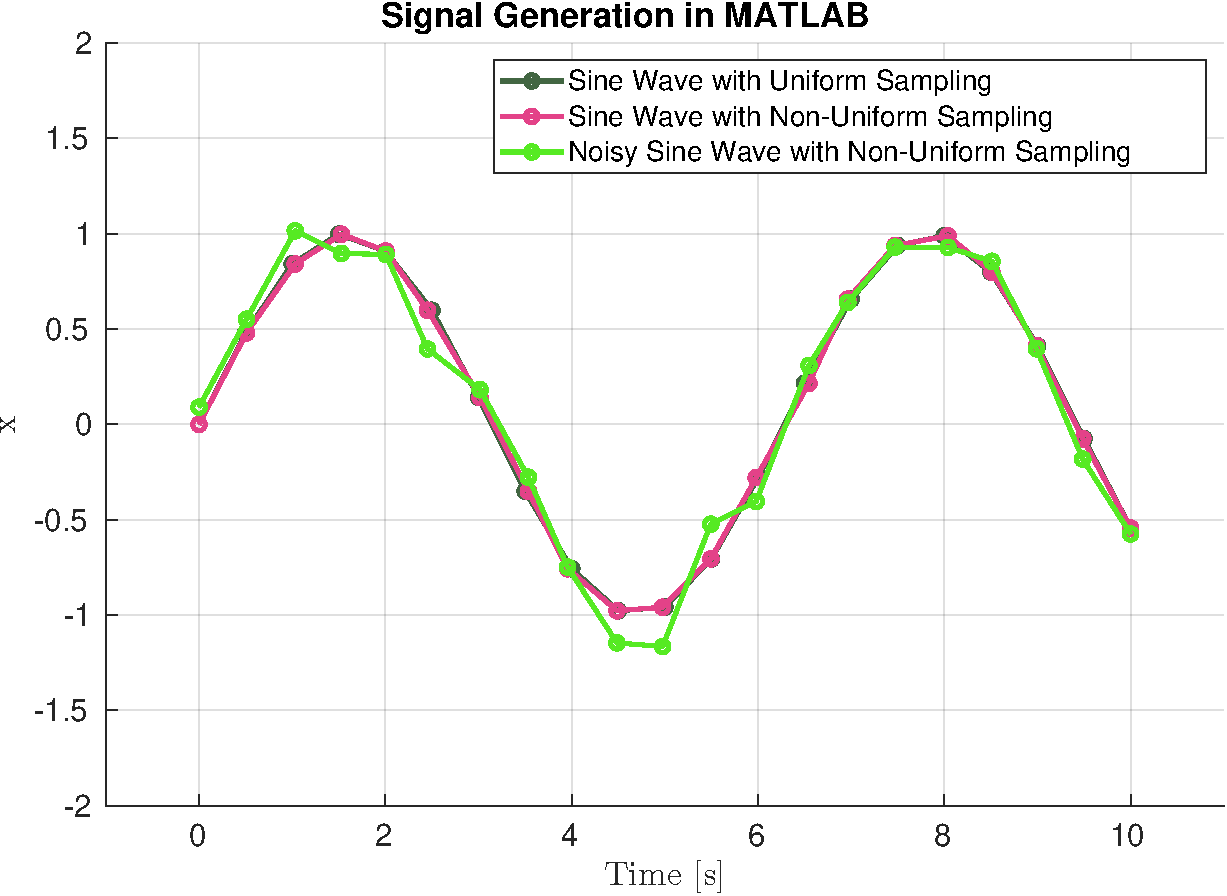
\includegraphics[width=0.6\linewidth]{../Code/figures/Ch02_signal_generation.pdf}

\footnotesize Full code: \url{https://github.com/rahulbhadani/CPE381_FA25/blob/main/Code/Ch02_Signal_Generation.m}
\end{center}

\end{frame}

\begin{frame}{Working with Real-life Signal}

\begin{itemize}
\item Real-life signals are noisy, i.e., not smooth, may not be differentiable at every time points.
\item May have high frequency noise -- usually due to another process 
\item May have low frequency noise -- may be due to missing data, packet drop, inefficiency acquisition of data
\item Non-uniform sampling time
\end{itemize}

\end{frame}

\begin{frame}{Example of Real-life Signal}

\begin{center}
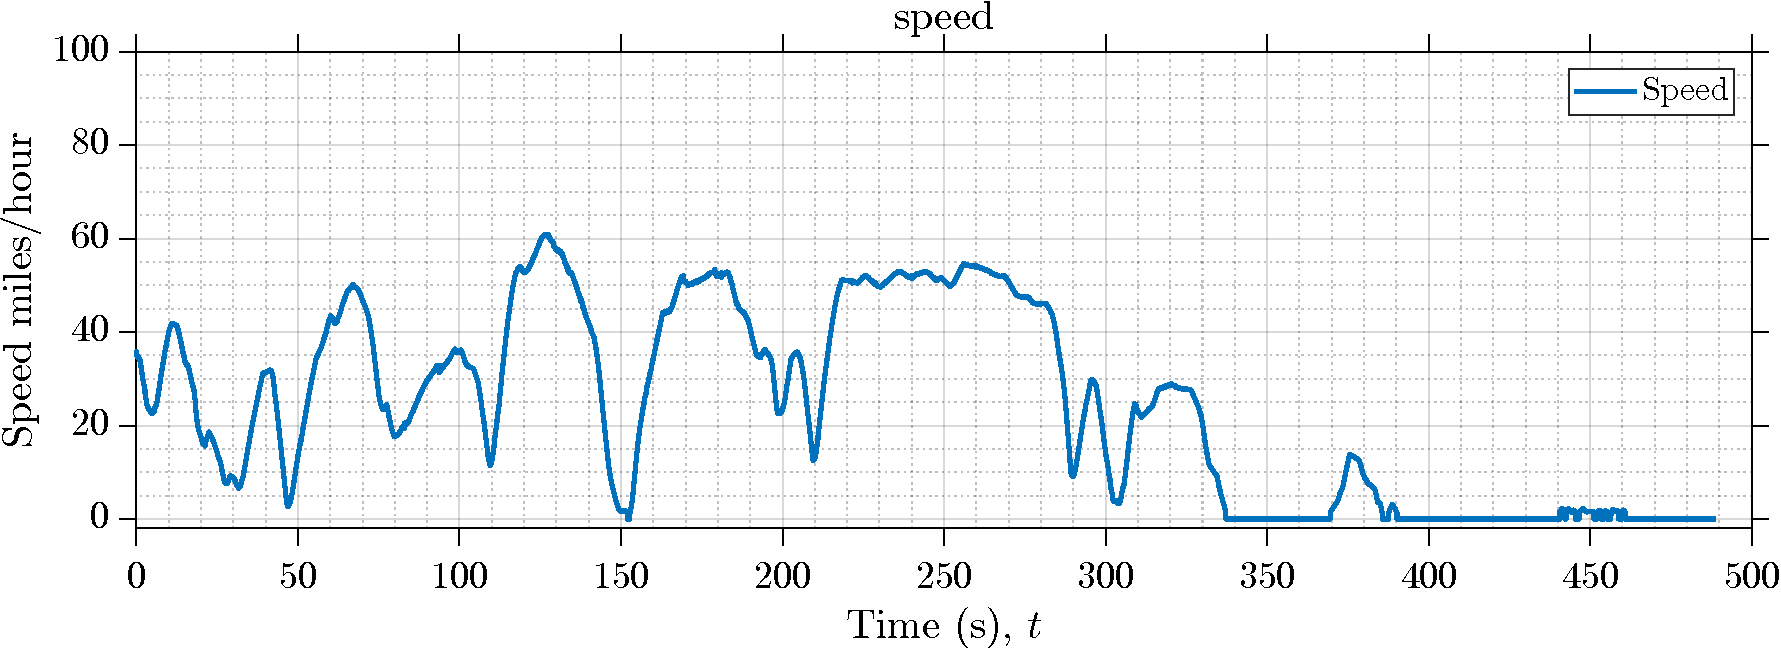
\includegraphics[width=0.5\linewidth]{../Code/figures/Ch02_reallife_speed.pdf}

\end{center}


\begin{columns}
\column{0.5\linewidth}

Histogram of $\Delta t$

\begin{center}
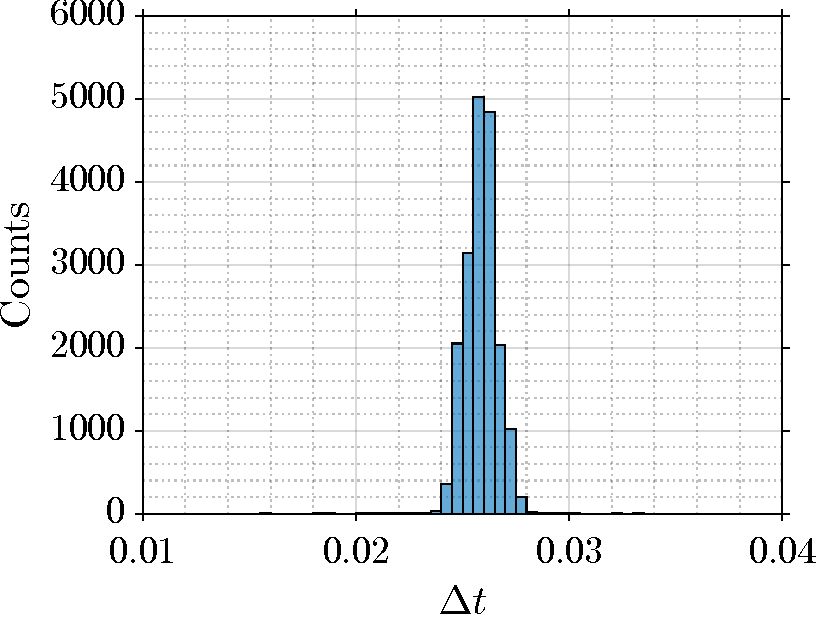
\includegraphics[width=0.5\linewidth]{../Code/figures/Ch02_reallife_speed_deltaT_Histogram.pdf}

\end{center}


\column{0.5\linewidth}

\begin{itemize}
\footnotesize
\item Speed data was collected from Toyota RAV4.
\item Mean $\Delta t = 0.025826$.

\item Code at \url{https://github.com/rahulbhadani/CPE381_FA25/blob/main/Code/Ch02_real_world_speed_data.m}
\item Data at \url{https://github.com/rahulbhadani/CPE381_FA25/blob/main/Data/vel.csv}
\end{itemize}

\end{columns}

\end{frame}


\begin{frame}{Pre-processing before we can use real-life Signals}

What do we want and what do we need to do?

What do we want?
\begin{itemize}

\item Signals at uniformly sampled time points.
\item Remove noise.
\item Resample at different sampling time or frequency.
\end{itemize}

What can we do to meet our requirements?

\begin{itemize}
\item Realign time points by assuming sampling time as constant, equal to mean sampling time.

\item Use interpolation methods for evaluation at new uniformly sampled points. Other techniques using frequency domain exists that we will study.

\item Removing noise is equivalent of smoothing signal data. We will learn in later chapters on smoothing a signal using new tools developed over the course of this semester.

\end{itemize}


\end{frame}


\begin{frame}{Interpolation Methods}


\begin{talert}{}
Interpolation finds the value between any two points based on some approximation by fitting a line or a curve.
\end{talert}

\begin{itemize}
\item We create uniformly sampled time-points, and approximate signal values at those points to create uniformly-sampled signals.
\end{itemize}


\end{frame}


\subsection{Linear Interpolation}

\begin{frame}
    \subsectionpage
\end{frame}

\begin{frame}{Linear Interpolation}
Two consecutive points are used to fit a line, and and a signal value is computed over an intermediate time point. The line is called \textbf{interpolant}.

\begin{columns}
\column{0.5\linewidth}
\begin{center}
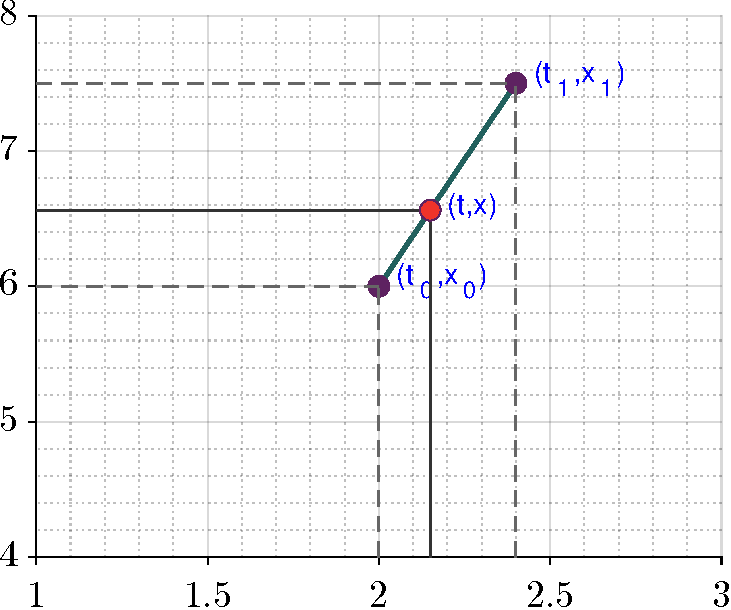
\includegraphics[width=0.75\linewidth]{../Code/figures/Ch02_line_equation.pdf}

\end{center}


\column{0.5\linewidth}

\footnotesize
\begin{itemize}
\item A line equation is $x = mt + c$, $m$ is the slope of the line, and $c$ is the intercept.

\item Two-point line equation can equivalently be written as $ x = x_0+ \cfrac{(x_1 - x_0)}{(t_1 - t_0)} (t - t_0)$  

\item $m = \cfrac{(x_1 - x_0)}{(t_1 - t_0)}$, $c = x_0 - m t_0$.

\item For every original consecutive time points $[t_k, t_{k+1}]$, compute the localized line equation, and then, for a new time points   $t_{k}\leq t\leq t_{k+1}$, compute the signal value $x$.
\end{itemize}
\end{columns}
\end{frame}

\begin{frame}{Linear Interpolation: Implementation in MATLAB}

\begin{center}

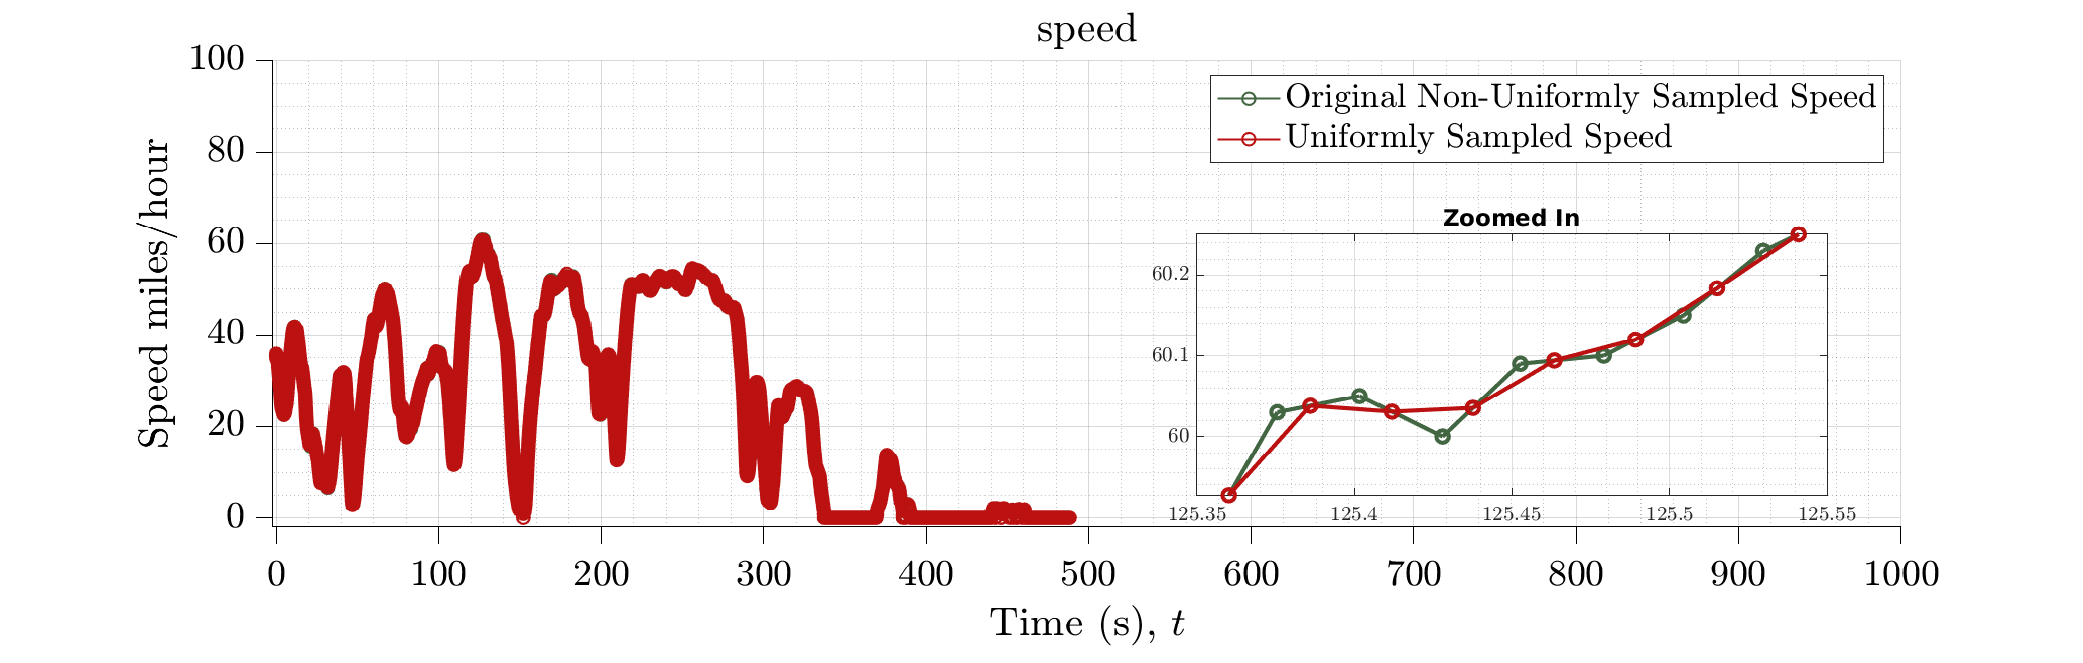
\includegraphics[width=1.0\linewidth]{../Code/figures/Ch02_Linear_Interpolation_Resampling.pdf}

\footnotesize 
Code: \url{https://github.com/rahulbhadani/CPE381_FA25/blob/main/Code/Ch02_Linear_Interpolation.m}
\end{center}
\end{frame}


\subsection{Cubic Spline Interpolation}

\begin{frame}
    \subsectionpage
\end{frame}


\begin{frame}{Cubic Spline Interpolation}
Instead of a line, we could fit a polynomial of degree $n+1$ using $n$ data points. However, we must limit to low-degree polynomials to avoid spurious approximations at new time-points.

\begin{peach}{}
\vspace{10pt}
\begin{center}
How many data points do we need to create a cubic spline interpolant?
\end{center}
\end{peach}

\end{frame}


\begin{frame}{Cubic Spline Interpolation}

Cubic function is $f(t) = at^3 + bt^2 + ct + d$. 

\vspace{10pt}

How do we choose coefficients $a, b, c, d$. 

\vspace{10pt}


We could use four successive points to fit a curve, but that won't give as smooth fit on the entire data.


\begin{center}
\Large Why?
\end{center}

\end{frame}


\begin{frame}{Cubic Spline Interpolation}
Consider interpolants at two successive points, $P_1(t)$ and $P_2(t)$.
\begin{center}
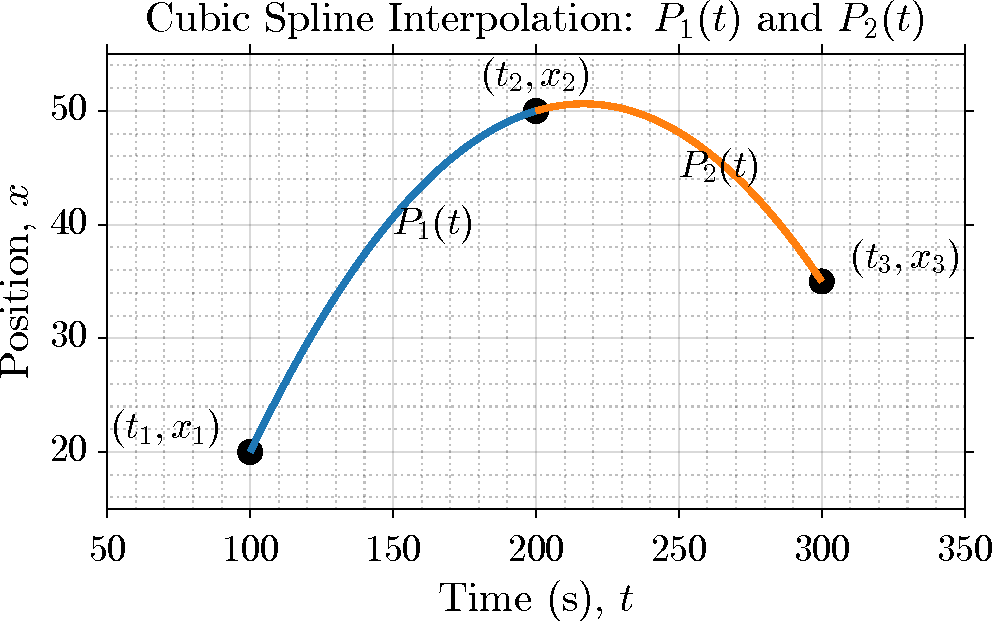
\includegraphics[width=0.4\linewidth]{../Code/figures/Ch02_CubicSpline_Segments.pdf}
\end{center}

\vspace{10pt}

How do we fit a curve of degree 3 with only two points?

\textbf{Answer:} We utilize continuity and smoothness that we desire at knot points. $(t_1, x_1), (t_2, x_2), \cdots $ are knot points.

\end{frame}

\begin{frame}{Cubic Spline Interpolation}

\footnotesize

We write $n$ cubic polynomails as $P_i(t) = a_i(t - t_i)^3 + b_i(t - t_i)^2 + c_i(t - t_i) + d_i$, $i=1, 2, \cdots, n$





We desire
\begin{enumerate}
\item $P_1'(t_2) = P_2'(t_2)$ at interior knots.

\item $P_1''(t_2) = P_2''(t_2)$ at interior knots.
\end{enumerate}

Consider $n+1$ data points: $(t_1, x_1), (t_2, x_2), \cdots, (t_{n+1}, x_{n+1})$
. We will have a total of $n$ interpolant.

Hence, to determine coefficient of two consecutive cubic spline interpolant $P_i(t)$ and $P_{i+1}(t)$, we need,



\begin{enumerate}
\item $P_1(t_1) = x_1$, $P_n(t_{n+1}) = x_{n+1}$
\item $P_{i+1}(t_{i+1}) = P_i(t_{i+1})$, $i = 1, 2, \cdots , n-1$
\item $P_i(t_i) = x_i, i = 2, 3, \cdots, n$
\item $P_i'(t_{i+1}) = P_{i+1}'(t_{i+1})$, $i = 1, 2, \cdots, n-1$
\item $P_i''(t_{i+1}) = P_{i+1}''(t_{i+1})$, $i = 1, 2, \cdots, n-1$

\end{enumerate}

A total of $4n-2$ equations. We also need boundary conditions.

\tiny Boundary conditions indicate the manner in which the first spline departs from the first data point and the last spline arrives at the last data point.

\end{frame}

\begin{frame}{Cubic Spline Interpolation}

\footnotesize

\textbf{Coefficient to determine:} $a_i, b_i, c_i, d_i$ for $i=1$ to $n$.
\begin{multiequation}
P_i(t) = a_i(t-t_i)^3 + b_i(t-t_i)^2 + c_i(t-t_i) + d_i
\end{multiequation}
Using this, we have:
\begin{multiequation}
P_i(t_i) = d_i = x_i
\end{multiequation}
Let $h_i = t_{i+1} - t_i$, the spacing between time points.
\end{frame}

\begin{frame}{Cubic Spline Interpolation}
\footnotesize

Using the second condition, we have:
\begin{multiequation}
P_{i+1}(t_{i+1}) = P_i(t_{i+1})
\end{multiequation}
\begin{multiequation}
d_{i+1} &= a_i(t_{i+1}-t_i)^3 + b_i(t_{i+1}-t_i)^2 + c_i(t_{i+1}-t_i) + d_i \\
d_{i+1} &= a_i h_i^3 + b_i h_i^2 + c_i h_i + d_i, \quad i=1, \dots, n-1
\end{multiequation}


If we define $d_{n+1}=y_{n+1}$, then
\begin{multiequation}
\label{eq:cubic_1}
d_{i+1} = a_i h_i^3 + b_i h_i^2 + c_i h_i + d_i, \quad  i=1, \dots, n
\end{multiequation}

\end{frame}

\begin{frame}{Cubic Spline Interpolation}
\footnotesize

Taking the first derivative of $P_i(t)$ and applying the 4th condition:
\begin{multiequation}
\label{eq:cubic_2}
c_{i+1} = 3a_ih_i^2 + 2b_ih_i + c_i, \quad i = 1, 2, \cdots, n-1
\end{multiequation}

If we define, $c_{n+1} = P'_(t_{n+1})$, then 
\begin{multiequation}
\label{eq:cubic_2A}
c_{i+1} = 3a_ih_i^2 + 2b_ih_i + c_i, \quad i = 1, 2, \cdots, n
\end{multiequation}

\end{frame}


\begin{frame}{Cubic Spline Interpolation}
\footnotesize

Taking the second derivative of $P_i(t)$ and applying the 5th condition:
\begin{multiequation}
\label{eq:cubic_3}
2b_{i+1} = 6a_i h_i + 2b_i\\
b_{i+1} = 3a_i h_i + b_i, \quad  i=1, \dots, n-1
\end{multiequation}
If we define $b_{n+1} = \frac{1}{2}P_n''(t_{n+1})$, then 
\begin{multiequation}
\label{eq:cubic_3A}
b_{i+1} = 3a_i h_i + b_i, \quad  i=1, \dots, n
\end{multiequation}


From this, we can express $a_i$ as:
\begin{multiequation}
\label{eq:cubic_4}
a_i = \frac{b_{i+1}-b_i}{3h_i}
\end{multiequation}
\end{frame}


\begin{frame}{Cubic Spline Interpolation}

\footnotesize

Putting Equation~\eqref{eq:cubic_4} into Equation~\eqref{eq:cubic_1} and Equation~\eqref{eq:cubic_2A}, we have, 
\begin{multiequation}
\label{eq:cubic_5}
d_{i+1} &= \frac{1}{3}(2b_{i}+ b_{i+1})h_i^2 + c_i h_i + d_i \quad i=1, \dots, n
\end{multiequation}

and

\begin{multiequation}
\label{eq:cubic_6}
c_{i+1} & = (b_i+ b_{i+1}) h_i + c_i,  \quad  i=1, \dots, n\\
c_i & = \frac{d_{i+1}-d_i}{h_i} - \cfrac{1}{3} (2 b_i + b_{i+1}) h_i
\end{multiequation}

Changing $i$ to ${i-1}$


\begin{multiequation}
\label{eq:cubic_6A}
c_{i-1} = \frac{d_{i}-d_{i-1}}{h_i} - \cfrac{1}{3} (2 b_{i-1} + b_{i}) h_{i-1}
\end{multiequation}

and from Equation~\eqref{eq:cubic_6}, 
\begin{multiequation}
\label{eq:cubic_7}
c_i = (b_{i-1} + b_i)h_{i-1} + c_{i-1}
\end{multiequation}

\end{frame}

\begin{frame}{Cubic Spline Interpolation}

\footnotesize

Using Equation~\eqref{eq:cubic_6}, and Equation~\eqref{eq:cubic_7}, we can write:

\begin{multiequation} 
\label{eq:cubic_8}
b_{i-1}h_{i-1} + 2b_i(h_i+h_{i-1}) + b_{i+1}h_i = 3\left(\frac{d_{i+1}-d_i}{h_i} - \frac{d_i-d_{i-1}}{h_{i-1}}\right), \quad i = 2, \cdots, n
\end{multiequation}

This describes a system of equations whose only uknowns are $b_i$.

\vspace{10pt}
However, Equation~\eqref{eq:cubic_8} generates a system of $(n-1)$ equations in $n+1$ unknowns ($b_1, \dots, b_{n+1}$). We need two more equations that come from boundary conditions.


\end{frame}

\begin{frame}{Cubic Spline Interpolation}

\footnotesize

$i=1$ gives 

\begin{multiequation} 
\label{eq:cubic_9}
c_1 = \frac{d_2-d_1}{h_1} - \frac{1}{3}(2b_1 + b_2)h_1
\end{multiequation}

We can have two kind of boundary conditions: (i) Clamped Boundary Conditions where $P_1'(t) = p$, and $P_n'(t) = q$; (ii) Free Boundary Conditions where  $P_1''(t) = 0$, and $P_n''(t) = 0$;

\end{frame}

\begin{frame}{Cubic Spline Interpolation}

\footnotesize

For \textbf{Clamped Boundary Conditions}, $c_1 = P_1'(t) = p$, then 

\begin{multiequation} 
\label{eq:cubic_10}
(2b_1 + b_2)h = \frac{3(d_2-d_1)}{h_1} - 3p
\end{multiequation}

From Equation~\eqref{eq:cubic_6}, 


\begin{multiequation} 
\label{eq:cubic_11}
c_{n+1} = (b_n + b_{n+1})h_n + c_n
\end{multiequation}
and from the boundary condition, 

\begin{multiequation} 
\label{eq:cubic_12}
c_{n+1} = P_n'(t_{n+1}) = q\\
c_n = q - (b_n + b_{n+1})h_n
\end{multiequation}

\end{frame}

\begin{frame}{Cubic Spline Interpolation}




\footnotesize

\underline{\textbf{Clamped Boundary Conditions}}

\vspace{10pt}

Equation~\eqref{eq:cubic_6}, when $i=n$,
\begin{multiequation} 
\label{eq:cubic_13}
c_{n} = \frac{d_{n+1} - d_n}{h_n}-\frac{1}{3}(2b_n + b_{n+1})h_n
\end{multiequation}

which gives
\begin{multiequation} 
\label{eq:cubic_14}
(2b_{n+1} + b_n)h_n = -\frac{3(d_{n+1} - d_n}{h_n} + 3q
\end{multiequation}


Together, Equation~\eqref{eq:cubic_8}, Equation~\eqref{eq:cubic_10}, and Equation~\eqref{eq:cubic_14} yield a system of $n+1$ equations in $n+1$ unknowns.

\end{frame}

\begin{frame}{Cubic Spline Interpolation}

\footnotesize

\underline{\textbf{Clamped Boundary Conditions}}

\vspace{10pt}

In summary:

\begin{enumerate}
\item $d_i = x_i, \quad i = 1, \cdots n$
\item $(2b_1 + b_2)h_1 = \frac{3(d_2 - d_1)}{h_1} - 3p$
\item $b_{i-1}h_{i-1} + 2b_i(h_i+h_{i-1}) + b_{i+1}h_i = 3\left(\frac{d_{i+1}-d_i}{h_i} - \frac{d_i-d_{i-1}}{h_{i-1}}\right), \quad i = 2, \cdots, n$
\item $(2 b_{n+1} + b_n) h_n = -\frac{d_{n+1} - d_n}{h_n} + 3q$
\end{enumerate}


\redcircle{2} and \redcircle{4} are single equation each, while \redcircle{3} generates $n-1$ equations.


\vspace{10pt}

Once $b_i$'s are known, we can find $c_i$'s using Equation~\eqref{eq:cubic_6}, and then using Equation~\eqref{eq:cubic_4}, we can find $a_i$'s. 


\end{frame}

\begin{frame}{Cubic Spline Interpolation}

\footnotesize

In Matrix Notation:

\begin{multiequation}
B\bbf & = \ybf\\
\begin{bmatrix}
2h_1 & h_1 & 0 & \cdots & 0 \\
h_1 & 2(h_1 + h_2) & h_2 & \cdots & 0 \\
0 & h_2 & 2(h_2 + h_3) & \cdots & 0 \\
\vdots & \vdots & \vdots & \ddots & \vdots \\
0 & \cdots & 0 & h_n & 2h_n
\end{bmatrix}\begin{bmatrix}
b_1 \\ b_2 \\ \vdots \\ b_{n+1}
\end{bmatrix} & = 3
\begin{bmatrix}
\dfrac{d_2 - d_1}{h_1} - p \\[12pt]
\dfrac{d_3 - d_2}{h_2} - \dfrac{d_2 - d_1}{h_1} \\[12pt]
\dfrac{d_4 - d_3}{h_3} - \dfrac{d_3 - d_2}{h_2} \\[12pt]
\vdots \\
q - \dfrac{d_{n+1} - d_n}{h_n}
\end{bmatrix}
\end{multiequation}

That we can solve in MATLAB to find \textbf{\texttt{b}} using \boxed{\texttt{\color{DarkBlue}B /\ y}}.


\end{frame}

\begin{frame}{Cubic Spline Interpolation}

\footnotesize

\underline{\textbf{Free Boundary Conditions}}

\vspace{10pt}

For free boundary conditions, $P_1''(t_1) = 0$, $P_n''(t_{n+1}) = 0$

Knowing, 
\begin{multiequation}
\label{eq:cubic_15}
P_1''(t) = 6a_1 (t - t_1) + 2b_1
\end{multiequation}
which yields $b_1 = 0$.

\vspace{10pt}

And, we get $b_{n+1} = \frac{1}{2}P_n''(t_{n+1})$ which implies $b_{n+1} = 0$.

In summary, 
\begin{enumerate}

\item $b_1 = 0$
\item $b_{i-1}h_{i-1} + 2b_i (h_i + h_{i-1}) + b_{i+1}h_i = \frac{3(d_{i+1} - d_i)}{h_i} - \frac{3(d_{i} - d_{i-1})}{h_{i-1}}$, $ i = 2, 3, \cdots n$
\item $b_{n+1} = 0$
\end{enumerate}

Once $b_i$'s are known, we can proceed in similar manner as described for finding coefficients for the case of \textbf{Clamped Boundation Conditions}.


\end{frame}


\begin{frame}{Cubic Spline Interpolation}

\footnotesize

In Matrix Notation:
\begin{multiequation}
B\bbf & = \ybf\\
\begin{bmatrix}
2(h_1+h_2) & h_2 & 0 & \cdots & 0 \\
h_2 & 2(h_2+h_3) & h_3 & \cdots & 0 \\
0 & h_3 & 2(h_3+h_4) & \cdots & 0 \\
\vdots & \vdots & \ddots & \ddots & \vdots \\
0 & 0 & \cdots & h_{n-1} & 2(h_{n-1}+h_n)
\end{bmatrix} \begin{bmatrix}
b_2 \\
b_3 \\
b_4 \\
\vdots \\
b_n
\end{bmatrix}
& =
\begin{bmatrix}
\frac{3(d_3-d_2)}{h_2} - \frac{3(d_2-d_1)}{h_1} \\
\frac{3(d_4-d_3)}{h_3} - \frac{3(d_3-d_2)}{h_2} \\
\frac{3(d_5-d_4)}{h_4} - \frac{3(d_4-d_3)}{h_3} \\
\vdots \\
\frac{3(d_{n+1}-d_n)}{h_n} - \frac{3(d_n-d_{n-1})}{h_{n-1}}
\end{bmatrix}
\end{multiequation}

Note that $b_1$ and $b_{n+1}$ are given as $0$, so they don't need to be solved for.

\end{frame}


\begin{frame}{MATLAB Implementation}

Example

Consider $t = [0, 1.01, 2.03, 3.01]$ and $x = [0, 0.5, 2, 1.5]$.

\vspace{10pt}


See the code for MATLAB function implementation: \url{https://github.com/rahulbhadani/CPE381_FA25/blob/main/Code/Ch02_cubic_spline_interpolation.m}

\vspace{10pt}

Demo usage: \url{https://github.com/rahulbhadani/CPE381_FA25/blob/main/Code/Ch02_demo_cubic_spline.m}

\vspace{5pt}

\tiny 
Reference: Numerical Methods for  Engineers and Scientists Using MATLAB, Second Edition,  Ramin S. Esfandiari

\end{frame}


\subsection{Differentiation in MATLAB}

\begin{frame}
    \subsectionpage
\end{frame}

\begin{frame}{Differentiation in MATLAB}



Differentiation in MATLAB is achieved through discrete derivation

\footnotesize

\begin{table}[h]
\centering
\caption{First Derivative Difference Formulas}
\begin{tabular}{ll}
\hline
\textbf{Difference Formula} & \textbf{First Derivative} \\
\hline
Two-point backward & $f'(x_i) = \frac{f(x_i) - f(x_{i-1})}{h}$ \\
Two-point forward & $f'(x_i) = \frac{f(x_{i+1}) - f(x_i)}{h}$ \\
Two-point central & $f'(x_i) = \frac{f(x_{i+1}) - f(x_{i-1})}{2h}$ \\
Three-point backward & $f'(x_i) = \frac{f(x_{i-2}) - 4f(x_{i-1}) + 3f(x_i)}{2h}$ \\
Three-point forward & $f'(x_i) = \frac{-3f(x_i) + 4f(x_{i+1}) - f(x_{i+2})}{2h}$ \\
Four-point central & $f'(x_i) = \frac{f(x_{i-2}) - 8f(x_{i-1}) + 8f(x_{i+1}) - f(x_{i+2})}{12h}$ \\ \\
\hline
\end{tabular}
\end{table}

Here, $x_i = x[i]$.

\end{frame}

\begin{frame}{Differentiation in MATLAB}

\footnotesize


\begin{table}[h]
\centering
\caption{Second Derivative Difference Formulas}
\begin{tabular}{ll}
\hline
\textbf{Difference Formula} & \textbf{Second Derivative} \\
\hline
Three-point backward & $f''(x_i) = \frac{f(x_{i-2}) - 2f(x_{i-1}) + f(x_i)}{h^2}$ \\
Three-point forward & $f''(x_i) = \frac{f(x_{i+2}) - 2f(x_{i+1}) + f(x_i)}{h^2}$ \\
Three-point central & $f''(x_i) = \frac{f(x_{i-1}) - 2f(x_i) + f(x_{i+1})}{h^2}$ \\
Four-point backward & $f''(x_i) = \frac{-f(x_{i-3}) + 4f(x_{i-2}) - 5f(x_{i-1}) + 2f(x_i)}{h^2}$ \\
Four-point forward & $f''(x_i) = \frac{2f(x_i) - 5f(x_{i+1}) + 4f(x_{i+2}) - f(x_{i+3})}{h^2}$ \\
Five-point central & $f''(x_i) = \frac{-f(x_{i-2}) + 16f(x_{i-1}) - 30f(x_i) + 16f(x_{i+1}) - f(x_{i+2})}{12h^2}$ \\ \\
\hline
\end{tabular}
\end{table}

\end{frame}

\begin{frame}[containsverbatim]{Differentiation in MATLAB: Example}

\Large 

    $$
    y(t) = \cos(t^2)
    $$
\end{frame}
\begin{frame}[containsverbatim]{Differentiation in MATLAB: Example}
    \footnotesize
\begin{columns}
    \column{0.5\linewidth}
    \begin{verbatim}
%% Solving derivatives symbolically
% y(t) = cos(t^2)
% dy/dt = -2*t*sin(t^2)
%% Symbolic derivative: the ground truth
syms t y z % we define symbols
y = cos(t^2);
z = diff(y);
figure(1);
subplot(2, 1, 1)
% symbolic plotting
fplot(y, [0, 2*pi], 'LineWidth', 3);
grid on;
hold on;
subplot(2, 1, 2);
fplot(z, [0, 2*pi], 'LineWidth', 3);
grid on;
hold on;
    \end{verbatim}
    \column{0.5\linewidth}
    \begin{verbatim}
%% Numerical derivative
Ts = 0.1;
t1 = 0:Ts:2*pi;
y1 = cos(t1.^2);
z1 = diff(y1)./diff(t1);
figure(1);
subplot(2, 1, 1);
stem(t1, y1, 'r');
subplot(2, 1, 2);
stem(t1(1:length(y1) -1), z1, 'm' );

    \end{verbatim}
\end{columns}
\end{frame}


\begin{frame}{Differentiation of a Real Signal}

\begin{center}
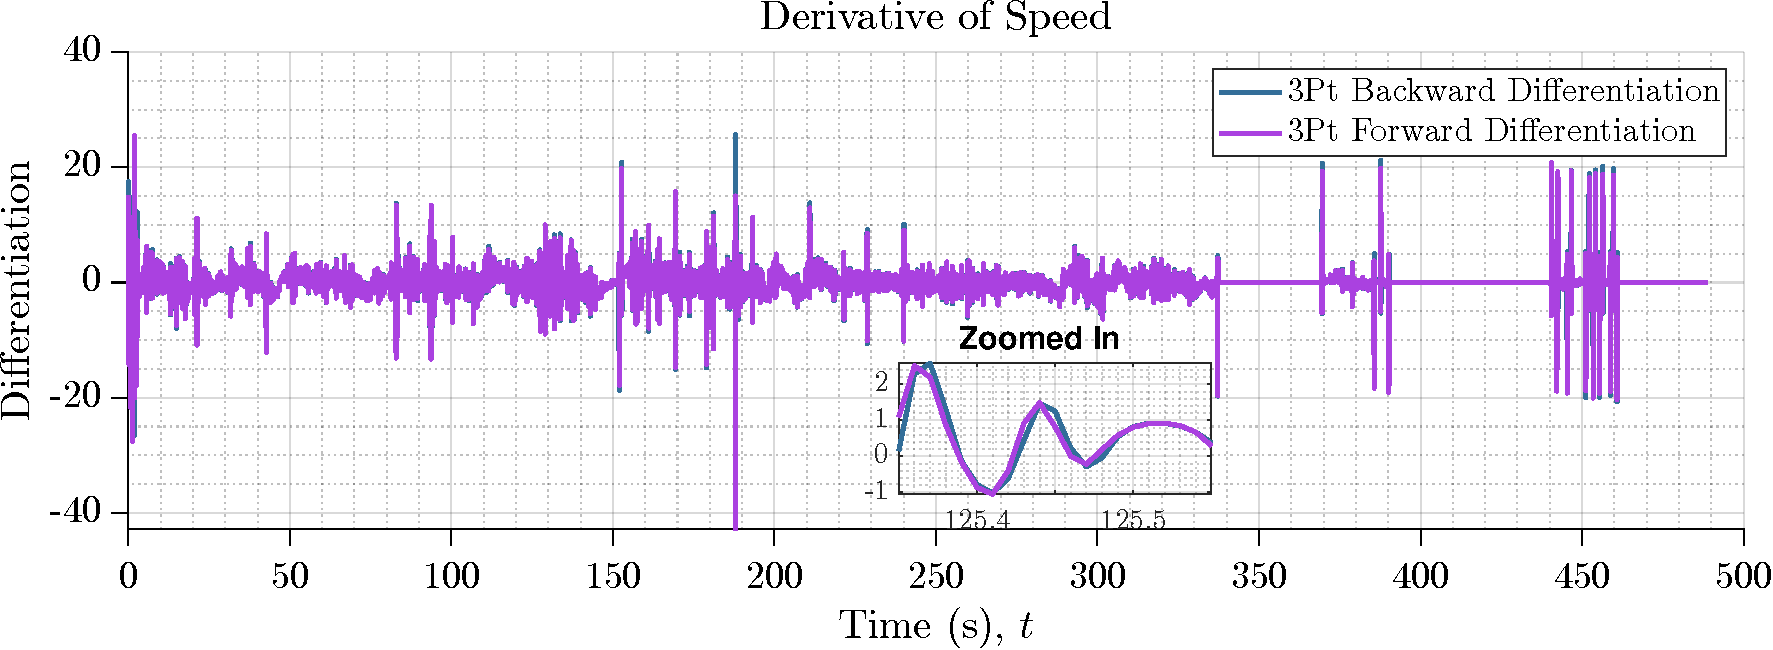
\includegraphics[width=0.9\linewidth]{../Code/figures/Ch02_Differentiation_Real_Signal.pdf}

\footnotesize

Code: 

\url{https://github.com/rahulbhadani/CPE381_FA25/blob/main/Code/Ch02_Differentiation_Real_Signal.m}

\end{center}

\end{frame}

\subsection{Integration in MATLAB}

\begin{frame}
    \subsectionpage
\end{frame}

\begin{frame}{Integration Example}

\footnotesize
    $$
    \int\cfrac{x^3}{x+2} dx
    $$

    \begin{multiequation}
  \int\frac{x^3}{x+2} dx &= \int\frac{x^3+8-8}{x+2} dx & \text{Add and subtract 8 to the numerator} \\
  &= \int\frac{(x+2)(x^2-2x+4)-8}{x+2} dx & \text{Factor the numerator} \\
  &= \int\left(x^2-2x+4-\frac{8}{x+2}\right) dx & \text{Split the fraction} \\
  &= \int x^2 dx - 2\int x dx + 4\int dx - 8\int\frac{1}{x+2} dx & \text{Split the integral into separate terms} \\
  &= \frac{x^3}{3} - x^2 + 4x - 8\ln|x+2| + C & \text{Evaluate each integral}
\end{multiequation}
\end{frame}

\begin{frame}[containsverbatim]{Integration in MATLAB}
    \small
    \begin{columns}
    \column{0.4\linewidth}
    \begin{verbatim}
%% Symbolic Integration
% x^3/(x + 2) dx
syms x
f = x^3/(x + 2)
% indefinite integral
int(f)
% definite integral
int(f, 0, 10)
    \end{verbatim}
    \column{0.6\linewidth}
    \begin{verbatim}
%% Numerical Integration using trapezoidal rule, 
%% Numerical integration is always definite
x = 0:0.1:10;
f = x.^3./(x + 2);
trapz(x, f)
    \end{verbatim}
\end{columns}
\end{frame}



\subsection{Solving Differential Equation in MATLAB}

\begin{frame}
    \subsectionpage
\end{frame}


\begin{frame}{Differential Equation: Initial Value Problems}

\begin{itemize}
\item An nth-order differential equation, requires $n$ conditions
\item When these conditions are provided at the same initial value of the independent variable, we have an \textbf{initial-value problem (IVP)}.
\end{itemize}

\vspace{10pt}

\begin{center}
A single, first-order initial-value problem is formulated as

\begin{multiequation}
\frac{dx(t)}{dt} = x(t), x(0) = x_0, 0\leq t \leq t_n
\end{multiequation}

\end{center}

\end{frame}

\begin{frame}{Solving Ordinary Differential Equations using Numerical Methods}
Recognizing that derivatives can be approximated as difference equations in the discrete domain, we have some methods to solve ordinary differential equations, suitable for computer implementations.

Some common numerical methods to solve ODE are:
\begin{itemize}
    \item Euler's Method
    \item Runge-Kutta Method (4th Order)
\end{itemize}
\end{frame}

\begin{frame}
\frametitle{Euler's Method}
\begin{itemize}
    \item Consider the ODE: $ \frac{dy}{dt} = f(t, y) $
    \item Initial condition: $ y(t_0) = y_0 $
    \item Euler's method formula: $ y_{n+1} = y_n + h f(t_n, y_n) $
    \item Example: $ \frac{dy}{dt} = -2y, \quad y(0) = 1 $
    \item Using $ h = 0.1 $: $ y_{n+1} = y_n - 0.2y_n = y_n(1 - 0.2) $
\end{itemize}
\end{frame}

\begin{frame}
  \frametitle{Euler's Method}
  \textbf{Euler's method:}
  \begin{equation*}
    y_{n+1} = y_n + hf(t_n, y_n)
  \end{equation*}
  
  \textbf{Example:} Solve $y' = 2t$ with $y(0) = 1$ using Euler's method with $h = 0.1$
  \begin{itemize}
    \item In this case, $f(t, y) = 2t$
  \end{itemize}
  \begin{table}
    \begin{tabular}{c|c|c}
      $t_n$ & $y_n$ & $y_{n+1}$ \\
      \hline
      0 & 1 & 1.0 \\
      0.1 & 1.0 & 1.02 \\
      0.2 & 1.02 & 1.06 \\
      \vdots & \vdots & \vdots
    \end{tabular}
  \end{table}
\end{frame}

\begin{frame}
\frametitle{Runge-Kutta Method (4th Order)}
\begin{columns}
    \column{0.5\linewidth}
    \begin{itemize}
          \item Consider the ODE: $ \frac{dy}{dt} = f(t, y) $
    \item Initial condition: $ y(t_0) = y_0 $
    \item Runge-Kutta method formula:
    $$
    \begin{aligned}
    k_1 &= h f(t_n, y_n) \\
    k_2 &= h f\left(t_n + \frac{h}{2}, y_n + h \frac{k_1}{2}\right) \\
    k_3 &= h f\left(t_n + \frac{h}{2}, y_n + h \frac{k_2}{2}\right) \\
    k_4 &= h f(t_n + h, y_n + h k_3) \\
    y_{n+1} &= y_n + \frac{1}{6}(k_1 + 2k_2 + 2k_3 + k_4)
    \end{aligned}
    $$
    \end{itemize}

\column{0.5\linewidth}
\begin{itemize}
  
    \item Example: $ \frac{dy}{dt} = t + y, \quad y(0) = 1 $
    \item Using $ h = 0.1 $:
   
    Write a MATLAB code to implement that.
\end{itemize}
\end{columns}
\end{frame}



\begin{frame}
  \frametitle{Runge-Kutta Methods}
  \textbf{Runge-Kutta methods:}
  \begin{itemize}
    \item More accurate than Euler's method
    \item Use multiple function evaluations at each step
  \end{itemize}
  \textbf{Example:} Solve $y' = 2x$ with $y(0) = 1$ using the Runge-Kutta method of order 4 with $h = 0.1$
  \begin{table}
    \begin{tabular}{c|c|c}
      $x_n$ & $y_n$ & $y_{n+1}$ \\
      \hline
      \vdots & \vdots & \vdots
    \end{tabular}
  \end{table}
\end{frame}


\begin{frame}{Ordinary Differential Equation in MATLAB}
Solve the initial value problem $ty' + 3y = 0, y(1) = 2$, assuming $t > 0$. We write the equation in standard form: $y' + 3y/t = 0$.

$$
P(t) = \int -\cfrac{3}{t}dt  = -3 \ln t
$$

and


$$
y = Ae^{-3\ln t} = At^{-3}
$$
Substitute to find $A$: $ 2= A(1)^{-3}$, so the solution is $y = 2t^{-3}$.
    
\end{frame}


\begin{frame}[containsverbatim]{Ordinary Differential Equation in MATLAB}
    \small
    \begin{verbatim}
%% ty; + 3y = 0; y(1) = 2
% solution y = 2/t^3
syms y(t)
eqn = diff(y, t) + 3*y/t ==0;
cond = y(1) == 2;
y(t) = dsolve(eqn, cond);
    \end{verbatim}
\end{frame}

\begin{frame}{Euler's Method Implementation}

Consider $t_0$ be the initial time, $h$ be the sampling time. Then $t_1 = t_0 + h$.

\vspace{10pt}

Using Taylor's Series:

\begin{multiequation}
x(t_1) & = x(t_0 + h) = x(t_0) + h x'(t_0)  + \cfrac{1}{2!}h^2 x''(t_0) + \cdots + \\
x(t_1) & \approx x(t_0) + h x'(t_0) 
\end{multiequation}

\end{frame}

\begin{frame}{Example and MATLAB Implementation of Euler ODE}

Consider $2x' + x(t) = e^{-t}, x(0) = 1/2, 0\leq t\leq 1$

\begin{center}

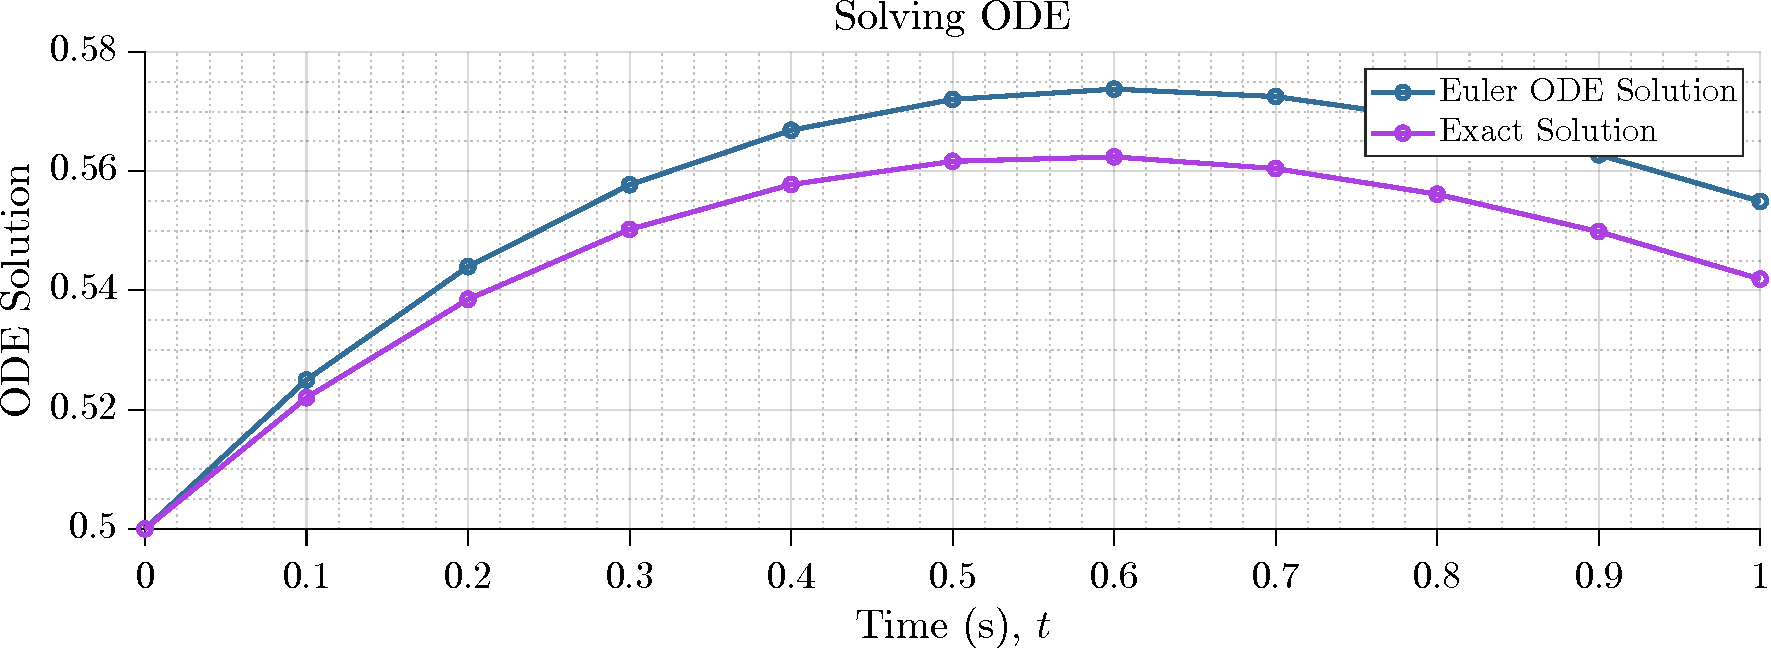
\includegraphics[width=0.9\linewidth]{../Code/figures/Ch02_demo_EulerODE.pdf}

\end{center}

\tiny



Code: 

\url{https://github.com/rahulbhadani/CPE381_FA25/blob/main/Code/Ch02_EulerODE.m}


\url{https://github.com/rahulbhadani/CPE381_FA25/blob/main/Code/Ch02_demo_EulerODE.m}


\end{frame}

\begin{frame}{Up Next}
\begin{itemize}
    \item Operations on Continuous-time Signals
\end{itemize}
    
\end{frame}

\end{document}